% =====================================================================
%  MODELO DE ARTIGO
%  Astronomia (AST0001) -- Curso de Física -- UDESC Joinville
%
%  COMO USAR
%   1. Preencha os campos marcados "PREENCHA AQUI", logo abaixo.
%   2. Escreva o conteúdo nas seções indicadas.
%   3. Compile com pdfLaTeX DUAS vezes (a segunda resolve as referências).
%
%  Linhas que começam com % são comentários: o LaTeX as ignora. Elas
%  explicam o que cada comando faz e o que se espera de cada seção.
%  Pode apagá-las na versão final.
% =====================================================================

\documentclass[10pt,a4paper,twocolumn]{article}

% ---------------------------------------------------------------- pacotes
\usepackage[utf8]{inputenc}
\usepackage[T1]{fontenc}
\usepackage[brazil]{babel}
\usepackage{amsmath,amssymb}
\let\Bbbk\relax                    % evita choque entre amssymb e newtxmath
\usepackage{newtxtext,newtxmath}   % tipografia de periódico (Times)
\usepackage{microtype}
\usepackage[a4paper,top=2.4cm,bottom=2.2cm,left=1.9cm,right=1.9cm,
            columnsep=0.7cm]{geometry}
\usepackage{graphicx}
\usepackage{booktabs}
\usepackage{siunitx}
\usepackage{caption}
\usepackage{titlesec}
\usepackage{fancyhdr}
\usepackage{xcolor}
\usepackage[colorlinks=true,linkcolor=udescverde,citecolor=udescverde,
            urlcolor=udescverde]{hyperref}

\definecolor{udescverde}{HTML}{1B6B3A}
\definecolor{cinza}{HTML}{5A5A5A}

\sisetup{output-decimal-marker={,}, per-mode=symbol}

% --------------------------------------------------- estilo das seções
\captionsetup{font=small,labelfont={bf,color=udescverde},labelsep=period}
\titleformat{\section}{\normalfont\bfseries\color{udescverde}}
            {\thesection.}{0.5em}{\MakeUppercase}
\titleformat{\subsection}{\normalfont\bfseries\itshape}{\thesubsection.}{0.5em}{}
\titlespacing*{\section}{0pt}{1.6ex}{0.8ex}
\setlength{\parindent}{1.2em}

% ---------------------------------------------------- PREENCHA AQUI
\newcommand{\titulo}{Título do artigo: uma frase que diz o que foi medido}
\newcommand{\aluno}{Nome Completo do Aluno}
\newcommand{\email}{email@edu.udesc.br}
\newcommand{\tituloCurto}{Título curto para o cabeçalho}
\newcommand{\semestre}{2026/2}
% -------------------------------------------------------------------

% ------------------------------------------------ cabeçalho das páginas
\pagestyle{fancy}
\fancyhf{}
\fancyhead[L]{\footnotesize\textcolor{cinza}{\aluno}}
\fancyhead[R]{\footnotesize\textcolor{cinza}{\tituloCurto}}
\fancyfoot[C]{\footnotesize\textcolor{cinza}{\thepage}}
\renewcommand{\headrulewidth}{0.3pt}
\fancypagestyle{primeira}{%
  \fancyhf{}\renewcommand{\headrulewidth}{0pt}
  \fancyfoot[C]{\footnotesize\textcolor{cinza}{\thepage}}}

\begin{document}

% =====================================================================
%  CABEÇALHO DA PRIMEIRA PÁGINA -- ocupa as duas colunas
% =====================================================================
\twocolumn[
\begin{@twocolumnfalse}

% tarja superior: identificação do periódico à esquerda, logo à direita
\noindent
\begin{minipage}{0.78\textwidth}
  {\footnotesize\textcolor{udescverde}{\textbf{ASTRONOMIA (AST0001)}}\\[2pt]
   \textcolor{cinza}{Universidade do Estado de Santa Catarina\, $\cdot$\,
   Centro de Ciências Tecnológicas\, $\cdot$\, Curso de Física}\\[2pt]
   \textcolor{cinza}{Joinville, \semestre}}
\end{minipage}
\hfill
\begin{minipage}{0.20\textwidth}
  \raggedleft{
\includegraphics[height=1.5cm]{udesc.png}}
\end{minipage}

\vspace{2pt}
{\color{udescverde}\rule{\textwidth}{1pt}}

\vspace{1.1em}
\begin{center}
  {\LARGE\bfseries \titulo\par}
  \vspace{0.9em}
  {\large \aluno\par}
  \vspace{0.3em}
  {\footnotesize\itshape\textcolor{cinza}{\email}\par}
  \vspace{0.3em}
  {\footnotesize\textcolor{cinza}{Recebido em \today}\par}
\end{center}

\vspace{0.9em}

% ------------------------------------------------------------ RESUMO
% O QUE ESCREVER: um parágrafo único, de 120 a 200 palavras, com
%   (i) contexto em uma frase, (ii) o que foi feito, (iii) que dados
%   foram usados, (iv) o RESULTADO NUMÉRICO principal, com incerteza,
%   (v) a conclusão em uma frase.
% O resumo é escrito POR ÚLTIMO, mas lido primeiro. Não cite equações
% nem figuras aqui, e não use referências.
\noindent\rule{\textwidth}{0.3pt}
\vspace{0.5em}

{\small
\noindent\textbf{Resumo.}
Escreva aqui o resumo em um único parágrafo. Comece dizendo qual pergunta
o trabalho responde e por que ela importa. Diga o que foi feito e com que
dados: quantas medidas, de que catálogo ou de que laboratório, com que
critério de seleção. Apresente o resultado principal em números, sempre
com incerteza e unidade --- por exemplo, ``obteve-se
$H_0 = 69 \pm 3\ \mathrm{km\,s^{-1}\,Mpc^{-1}}$''. Termine com uma frase
dizendo o que esse número significa e qual é a maior limitação da medida.
Um resumo bem escrito permite que o leitor decida, em trinta segundos, se
precisa ler o resto.

\vspace{0.6em}
\noindent\textbf{Palavras-chave:} três a cinco termos, separados por
travessão --- astronomia observacional --- fotometria --- paralaxe
}

\vspace{0.5em}
\noindent\rule{\textwidth}{0.3pt}
\vspace{1.4em}

\end{@twocolumnfalse}
]
\thispagestyle{primeira}

% =====================================================================
\section{Introdução}
% =====================================================================
% O QUE ESCREVER AQUI (2 a 4 parágrafos):
%   - do que trata o artigo e por que o assunto importa;
%   - o que já se sabe, com referência: \cite{carroll};
%   - a pergunta específica que ESTE artigo responde;
%   - como o texto está organizado.

Escreva aqui a apresentação do assunto. Situe o problema físico e diga por
que ele é interessante. Use referências para o que já é conhecido, como em
\cite{carroll}, e reserve para o final do texto o que é resultado seu.

O último parágrafo anuncia a estrutura: a Seção~\ref{sec:teoria} reúne as
relações usadas, a Seção~\ref{sec:dados} apresenta os dados e a análise, e
a Seção~\ref{sec:conclusao} discute o alcance e os limites do resultado.

% =====================================================================
\section{Revisão Teórica}
\label{sec:teoria}
% =====================================================================
% O QUE ESCREVER AQUI:
%   - apenas as equações que você vai usar de fato;
%   - o significado de cada símbolo;
%   - as hipóteses que cada equação assume.
% Regra prática: equação que não é usada na Seção 3 não entra aqui.

O fluxo recebido de uma fonte isotrópica cai com o quadrado da distância,
\begin{equation}
    F = \frac{L}{4\pi d^{2}},
    \label{eq:inverso}
\end{equation}
em que $F$ é o fluxo, $L$ a luminosidade e $d$ a distância. A
Equação~\eqref{eq:inverso} supõe emissão isotrópica e meio transparente.

% Como citar: \eqref{rótulo} produz "(1)" com os parênteses e atualiza
% o número sozinho se você inserir outra equação antes.
Comparando o fluxo observado ao que a mesma fonte teria a $10\,\mathrm{pc}$
obtém-se o módulo de distância:
\begin{align}
    m - M &= -2{,}5\log_{10}\left(\frac{10\,\mathrm{pc}}{d}\right)^{2}
    \nonumber \\
          &= 5\log_{10}\left(\frac{d}{\mathrm{pc}}\right) - 5.
    \label{eq:modulo}
\end{align}

% Equação sem numeração: use o ambiente com asterisco.
Quando há poeira no caminho, soma-se o termo de extinção $A$, e a relação
de trabalho passa a ser
\begin{equation*}
    m - M = 5\log_{10}d - 5 + A .
\end{equation*}

Símbolos no meio da frase vão entre cifrões, e valores com unidade saem
melhor com o comando \verb|\SI|: a paralaxe de Proxima Centauri vale
$p = \SI{768}{mas}$, o que corresponde a $d = \SI{1.30}{pc}$.

% =====================================================================
\section{Dados e Discussão}
\label{sec:dados}
% =====================================================================
% O QUE ESCREVER AQUI:
%   - origem dos dados: catálogo, laboratório, número de medidas,
%     critério de seleção;
%   - o tratamento aplicado;
%   - as figuras e tabelas, TODAS citadas no texto;
%   - o resultado numérico com incerteza e unidade;
%   - a comparação com o valor esperado e a discussão dos desvios.

Descreva a origem dos dados e o critério de seleção. Diga quantas medidas
sobraram e por quê.

% ------------------------------------------------ TABELA (uma coluna)
% Estrutura: table -> caption -> label -> tabular
%   {lccc} = uma letra por coluna: l esquerda, c centro, r direita
%   & separa colunas   \\ termina a linha
%   \toprule \midrule \bottomrule vêm do pacote booktabs
% Para acrescentar uma linha, copie uma linha e edite. Para acrescentar
% uma coluna, some uma letra em {lccc} e um & em cada linha.
A Tabela~\ref{tab:estrelas} traz a amostra analisada.

\begin{table}[t]
    \centering
    \caption{Paralaxe, distância e magnitude absoluta de quatro estrelas
             próximas. As distâncias vêm de $d=1/p$ e as magnitudes
             absolutas da Equação~\eqref{eq:modulo}.}
    \label{tab:estrelas}
    \small
    \begin{tabular}{lccc}
        \toprule
        Estrela & $p$ (mas) & $d$ (pc) & $M_G$ \\
        \midrule
        Proxima Centauri   & $768{,}07$ & $1{,}302$ & $15{,}5$ \\
        Estrela de Barnard & $546{,}98$ & $1{,}828$ & $13{,}9$ \\
        Wolf 359           & $415{,}18$ & $2{,}409$ & $16{,}1$ \\
        Lalande 21185      & $392{,}75$ & $2{,}546$ & $11{,}5$ \\
        \bottomrule
    \end{tabular}
\end{table}

% ------------------------------------------------ FIGURA (uma coluna)
% width=\linewidth ocupa a largura da COLUNA.
% A legenda vai sempre ABAIXO da figura.
A Figura~\ref{fig:hr} mostra o diagrama cor-magnitude da amostra.

\begin{figure}[t]
    \centering
    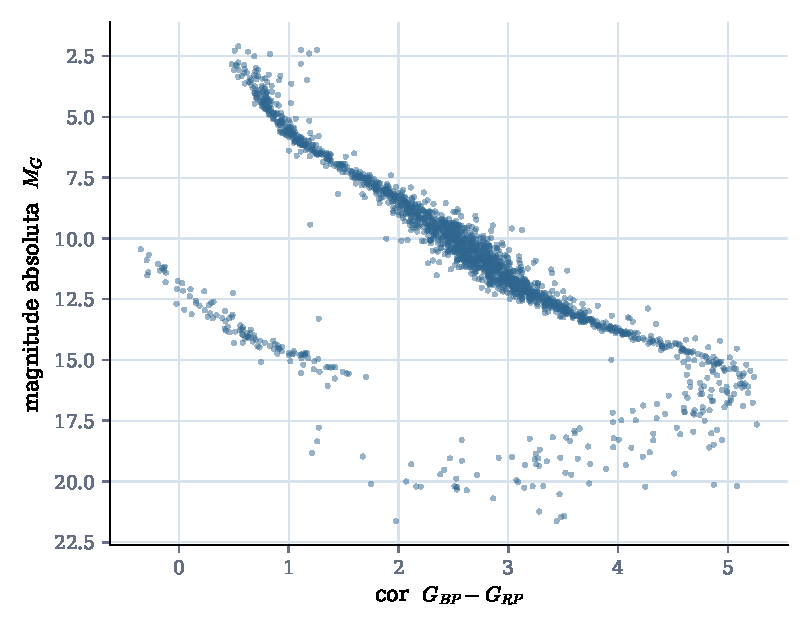
\includegraphics[width=\linewidth]{figura_exemplo.pdf}
    \caption{Diagrama cor-magnitude de estrelas a menos de
             \SI{25}{pc} do Sol, com dados da missão Gaia. O eixo vertical
             está invertido para que as mais luminosas fiquem em cima.}
    \label{fig:hr}
\end{figure}

% ------------------------------------ FIGURA LARGA (duas colunas)
% Para uma figura que ocupe a página inteira, use figure* em vez de
% figure e \textwidth em vez de \linewidth. Ela aparecerá no topo de
% uma página, não necessariamente aqui. Descomente para usar:
%
% \begin{figure*}[t]
%     \centering
%     \includegraphics[width=0.85\textwidth]{sua_figura_larga.pdf}
%     \caption{Legenda da figura larga.}
%     \label{fig:larga}
% \end{figure*}

Discuta o que a figura mostra. Aponte a estrutura principal, as exceções e
o que elas significam fisicamente. Evite descrever o gráfico em palavras
--- o leitor está vendo o gráfico; o que ele não vê é a sua interpretação.

O resultado principal deve aparecer destacado, com incerteza e unidade:
\begin{equation}
    H_0 = 69 \pm 3\ \mathrm{km\,s^{-1}\,Mpc^{-1}},
    \label{eq:resultado}
\end{equation}
em que a incerteza citada é apenas estatística. Compare com o valor de
referência e diga se a diferença é compatível: uma discrepância de
$2\sigma$ pede explicação; uma de $0{,}5\sigma$, não.

% =====================================================================
\section{Conclusão}
\label{sec:conclusao}
% =====================================================================
% O QUE ESCREVER AQUI:
%   - o que os números significam fisicamente;
%   - a maior fonte de incerteza, e se é estatística ou sistemática;
%   - o que uma medida melhor exigiria.
% NÃO repita a introdução e NÃO apresente resultado novo aqui.

Retome o resultado da Equação~\eqref{eq:resultado} e diga o que ele
significa. Identifique a etapa que domina a incerteza: é mais informativo
escrever ``a incerteza vem da calibração de distância, não da fotometria''
do que listar genericamente fontes de erro.

Termine dizendo o que seria necessário para melhorar a medida: mais dados,
outro instrumento, ou uma hipótese diferente no modelo.

% =====================================================================
%  BIBLIOGRAFIA
% =====================================================================
% Liste apenas o que você consultou de fato. No texto, cite com
% \cite{rótulo} -- por exemplo: \cite{gaia}.
\begin{thebibliography}{9}
\small

\bibitem{carroll}
CARROLL, B. W.; OSTLIE, D. A.
\textit{An Introduction to Modern Astrophysics}.
2. ed. Cambridge: Cambridge University Press, 2017.

\bibitem{apostila}
LIMA, R. C. R. de.
\textit{Astrofísica Moderna: capítulos de estudo}.
UDESC, 2026. Disponível em:
\url{https://rafaelcrdelima.github.io/Astronomia/}.

\bibitem{gaia}
GAIA COLLABORATION.
\textit{Gaia Data Release 3}. ESA, 2022. Disponível em:
\url{https://gea.esac.esa.int/archive/}.

\end{thebibliography}

\end{document}
